\chapter{研究の背景}
\label{chap:background}

本章ではまず提案手法の核となる技術であるDVFS、及びDVFSを用いた既存の電力削減手法について説明する。そして、対象とする蓄電池を含んだシステムの電力供給システムについて説明した後、蓄電池とDVFSの両方を用いた電力削減手法の関連研究を紹介する。

\section{DVFS}
\label{sec:dvfs}

\subsection{DVFSとは}

基本的に、プロセッサやメモリはある一定の周波数で動作するように設計されている。動作周波数が高いほど処理能力も高くなるが、同様に消費電力も大きくなる。そのため、プロセッサやメモリを省電力化する最も単純な手法の一つとして、動作周波数を低くするというものがある。かつてのプロセッサやメモリは設計時に決められた一つの動作周波数でしか動作することはできなかったが、現在では一つのプロセッサやメモリが複数の動作周波数をサポートしており、演算中であっても瞬時に動作周波数を切り替えられるようになった。この技術を用いて動的に動作周波数を切り替え、処理速度と消費電力を変化させることによって省電力化を行う手法をDVFS(Dynamic Voltage and Frequency Scaling)と呼ぶ。

図\ref{fig:dvfs_background}に、あるサーバプロセッサにおいてDVFSを用いたときの電力削減のグラフを示す\cite{Hennessy:2011:CAF:1999263}。動作周波数を低くすることにより処理できる最大負荷(Computer load)は下がるが、電力を削減することもできている。つまり、処理できる負荷であれば低い動作周波数の方が消費電力を少なくすることができる。図\ref{fig:dvfs_background}のDVS savingsの推移を見れば分かるように、この例ではDVFSを用いることにより最大で20\%ほどの電力削減が行えることになる。
\begin{figure}[t]
 \begin{center}
  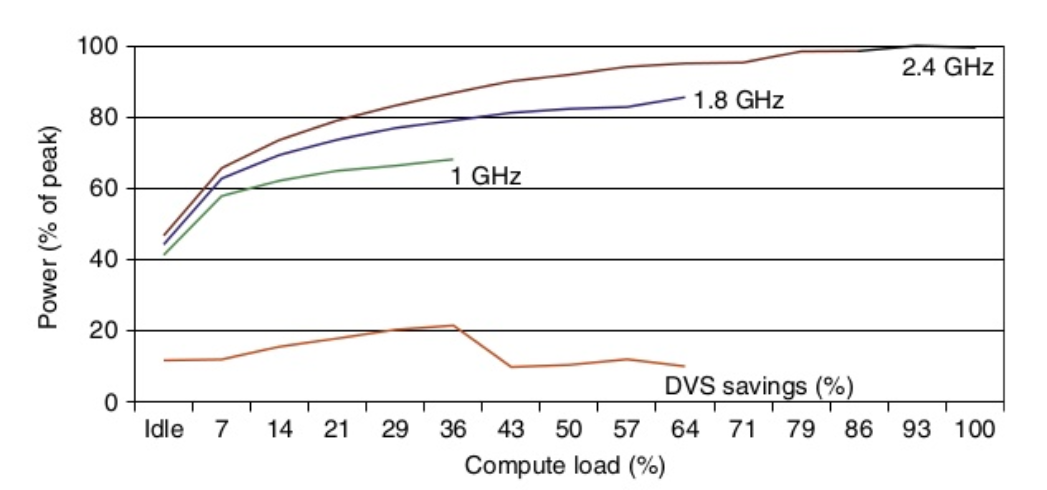
\includegraphics[width=110mm]{DVFS_background.png}
 \end{center}
 \caption{DVFSによる電力削減(AMD Opetron microprocessor) 文献\cite{Hennessy:2011:CAF:1999263} Figure 1.12より}
 \label{fig:dvfs_background}
\end{figure}


\subsection{DVFSを用いたコンピュータの既存の省電力化手法}

プログラム実行時、メモリやネットワークなどのプロセッサ以外のモジュールがボトルネックとなっているときには、プロセッサはビジーループとなり、処理を行わず電力だけを消費している時間の割合が高くなる。そのためこのような状況ではプロセッサ自体の処理能力を落としてもシステム全体の処理能力はあまり下がらないため、プロセッサを低い動作周波数に切り替えることで性能低下を防ぎつつ省電力化を行ってきた。

同様に、メモリがボトルネックとなっていない状態ではメモリの動作周波数を落とすことで電力を削減することができる\cite{David:2011:MPM:1998582.1998590}。

また、近年では複数のプロセッサを搭載したマルチプロセッサシステムが増えてきた。マルチプロセッサシステムは複数のプロセッサで並列に処理を行うことで高速化をはかっている。しかし、ひとつずつ順番に処理を行うことが必要なプログラムではひとつのプロセッサのみが処理を行っており、その他のプロセッサはほとんど処理を行っておらず、無駄な消費電力が発生していた。そのような状況では、処理を行っているひとつのプロセッサのみを高い周波数で動作させ、その他のプロセッサの動作周波数を落とすことで消費電力を削減している。

DVFSという技術は登場してからまだ日が浅く、DVFSを用いた電力削減や電力対性能向上の研究は現在盛んに行われている。例えば、2008年の研究では、複数プロセッサの組み込みシステムにおいてナノ秒単位でDVFS制御を行うことにより既存のDVFS制御からさらに20\%もの電力削減が行えるとされている\cite{4658633}。2011年の研究によると、メモリのバンド幅の使用率を用いてメモリのDVFS制御を行うことにより、システム全体のエネルギーの2.4\%を削減できる\cite{David:2011:MPM:1998582.1998590}。これ以外にも多くの研究がなされているが、それでもまだまだ多くの課題が残されているのが現状である。

\subsection{プロセッサとメモリのDVFSと組み合わせた電力削減の関連研究}

一般に、プログラム実行時はプロセッサかメモリのどちらかの処理能力がシステム全体のボトルネックとなっていることが多く、このときボトルネックとなっていないモジュールでは処理能力が必要以上に高い状態となっており、電力が無駄に消費されている。そのため、それぞれのモジュール間での処理能力の差をなくすことが、無駄な電力消費を減らす上で重要である。

この問題を解決するため、プロセッサとメモリのDVFSを同時に用いることによって、それぞれのDVFSを別々に行う場合よりもさらに電力対性能の向上を目指した手法が存在する\cite{6493615}。この手法では、5ミリ秒おきにプロセッサとメモリの処理能力の両方を監視して、一方のモジュールの処理能力が足りないときにはそのモジュールに電力を融通することによって処理能力の偏りをなくし、与えられた性能制約を満たしつつ省電力化を行っている。



\section{蓄電池を含む電力供給システム}
\label{sec:ups}

スーパーコンピュータやデータセンタなどの大規模高性能計算システムにおいては、高い信頼性が要求されるため、一瞬たりとも電圧低下や電力供給停止は許されない。そのため、停電や機器の故障によって電力会社からの電力供給が受けられない時にも、コンピュータへの電力供給を継続するためにいくつかの冗長電源設備が用意されている。現在のデータセンタの一般的な電源設備は図\ref{fig:power_distribution_background}のようになっている。
\begin{figure}[t]
 \begin{center}
  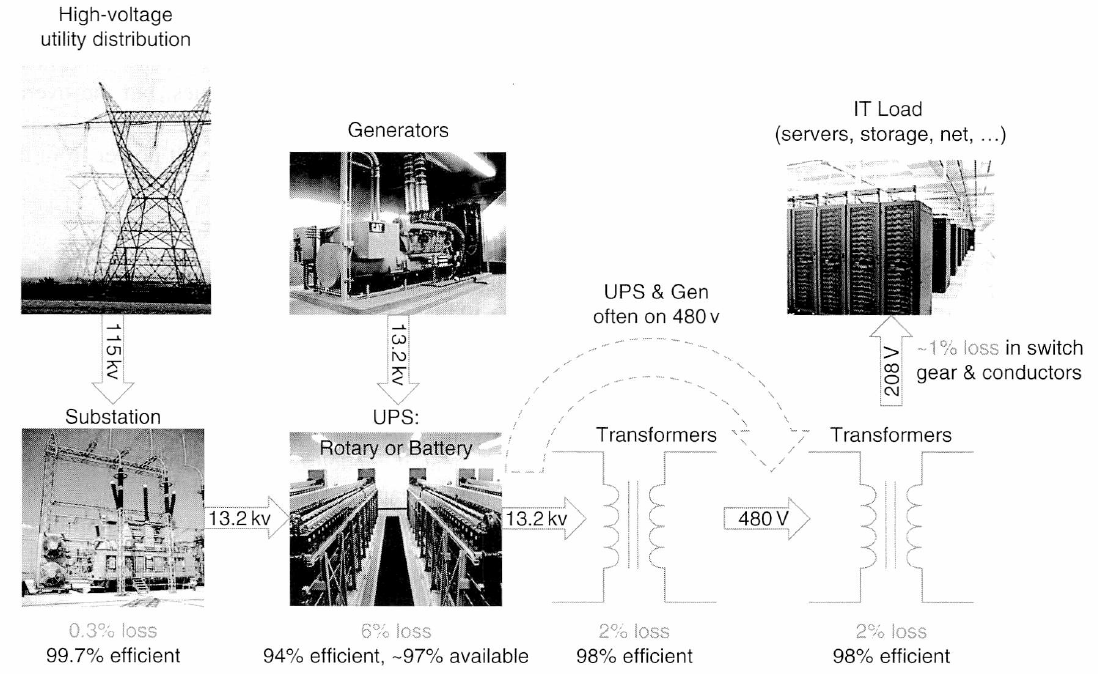
\includegraphics[width=120mm]{power_distribution_background.png}
 \end{center}
 \caption{データセンタにおける電源設備 文献\cite{Hennessy:2011:CAF:1999263} Figure 6.9より}
 \label{fig:power_distribution_background}
\end{figure}

電力会社からの電力供給が停止した場合には、UPS(無停電電源装置)が電力供給を行い、同時に自家発電設備が起動する。数分後、自家発電設備が完全に起動して電力供給が可能になると、自家発電設備から電力供給が行われるようになる。電力会社からの電力供給が再開すると自家発電設備は停止し、電力会社からの電力を使用するようになる。

ここでUPSは3つの役割を担っている。一つ目は、コンピュータへの供給電圧を安定させること。二つ目は、停電時に自家発電設備からの電力供給が始まるまでの間、電力を供給すること。三つ目は、停電復帰後に自家発電設備から電力会社に電力供給元を切り替えるとき、一時的に電力供給を行うことである。

UPS単体がシステム全体に電力を供給し続けられる時間は数分〜30分程度である場合が多い。現在の多くのUPSでは電源として蓄電池が使用されているが、充放電が行われるのは基本的に停電時のみであり、今のところ平常時に積極的に充放電を行うような使い方はなされていない。


\section{データセンタにおける蓄電池を用いたピーク電力削減手法}
\label{sec:capping}

前節\ref{sec:ups}で述べたように、今までは平常時に積極的にUPSの蓄電池から充放電を行うことはなかったが、2011年に発表された論文\cite{Govindan:2011:BLT:2024723.2000105}において、UPSからの充放電を用いたデータセンタの電力ピークカット手法が提案された。本稿の提案手法と大きく関わる内容であるので、ここで詳しく紹介する。

データセンタにおいてはコンピュータでの消費電力や冷却にかかる電力コストは全体の運用コストの10〜30\%に上り、サービス向上のために電力コストの削減が必要とされている。電力会社との契約料金はピーク時の電力に大きく影響される。そのためピーク電力を削減すべく、この論文ではUPSの中の蓄電池を用いた電力ピークカット手法を提案している。

データセンタの1日の電力需要の推移は、統計や過去の研究によってある程度予測ができるようになっている。その電力需要曲線から最適な蓄電池の充放電計画を立て、電力会社から引き込む電力の最大値を低く抑えることがこの紹介論文の主旨である(図\ref{fig:power_graph_datacenter})。
\begin{figure}[t]
 \begin{center}
  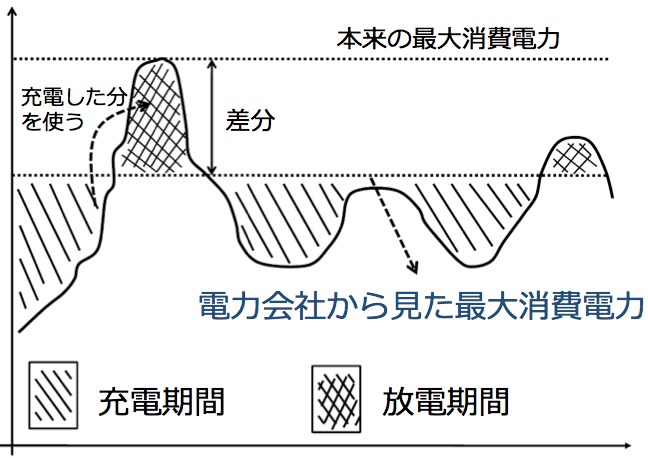
\includegraphics[width=90mm]{power_graph_datacenter.png}
 \end{center}
 \caption{蓄電池を用いた電力ピークカット手法}
 \label{fig:power_graph_datacenter}
\end{figure}

紹介論文において対象とする問題は以下のようになる。





Power Cappingの先行研究~\cite{Fan:2007:PPW:1273440.1250665}.
